\documentclass[aspectratio=169,10pt]{beamer}

\usepackage{minted}
\usepackage{tikz}
\usetikzlibrary{arrows,arrows.meta,bending,positioning,calc,patterns,backgrounds,fit,decorations.pathreplacing,shapes.geometric,shapes.multipart}
\usepackage{pdfpages}
\usepackage[detect-all,binary-units]{siunitx}
\usepackage{afterpage}
\usepackage{amsmath}
\usepackage{stmaryrd}
\usepackage{color}
\usepackage{transparent}
\usepackage{graphics}
\usepackage[section]{placeins}
\usepackage{subcaption}
\usepackage{sidecap}
\sidecaptionvpos{figure}{p}
\usepackage{tabularx}
\usepackage{booktabs}
\usepackage{adjustbox}
\usepackage{multirow}

\definecolor{color0}{HTML}{000000}
\definecolor{color1}{HTML}{E69F00}
\definecolor{color2}{HTML}{56B4E9}
\definecolor{color3}{HTML}{009E73}
\definecolor{color4}{HTML}{F0E442}
\definecolor{color5}{HTML}{0072B2}
\definecolor{color6}{HTML}{D55E00}
\definecolor{color7}{HTML}{CC79A7}

\setminted{fontsize=\footnotesize}

\newcommand*{\img}[1]{%
    \raisebox{-.3\baselineskip}{%
        \includegraphics[
        height=\baselineskip,
        width=\baselineskip,
        keepaspectratio,
        ]{#1}%
    }%
}

\definecolor{ao(english)}{rgb}{0.0, 0.5, 0.0}

\usepackage{appendixnumberbeamer}

\usepackage{listings}

\lstset{
	basicstyle=\footnotesize\ttfamily,
	emph={vector_fractional},emphstyle={\color{blue}},
}

\usepackage{siunitx}
\DeclareSIUnit\operation{op}
\newcommand{\der}[1]{\text{d} #1}

\newcommand{\tauref}[0]{\tau_{\text{ref}}}
\newcommand{\tausyn}[0]{\tau_{\text{syn}}}
\newcommand{\tauon}[0]{\tau_{\text{on}}}

\newcommand{\nunet}[0]{\nu^{\text{net}}}
\newcommand{\nutarget}[0]{\nu^{\text{target}}}
\newcommand{\nupre}[0]{\nu^{\text{pre}}}
\usepackage{letltxmacro}\LetLtxMacro{\cite}{\parencite}

\newcommand{\checkbox}[0]{\makebox[0pt][l]{$\square$}\raisebox{.15ex}{\hspace{0.1em}$\checkmark$}}
\newcommand{\nocheckbox}[0]{\makebox[0pt][l]{$\square$}\raisebox{.15ex}{\hspace{0.1em}{\transparent{0.0}{$\checkmark$}}}}

\usetheme[numbering=counter]{metropolis}

\title{Towards HTM on BrainScaleS-2}
\author{Robin Dietrich \& Philipp Spilger}

\begin{document}
\setbeamercolor{background canvas}{bg=white}

\setbeamertemplate{footline}[text line]{}

\setbeamertemplate{footline}[text line]{%
\raisebox{0.2cm}{\footnotesize\insertshortauthor}\hfill\raisebox{0.2cm}{\footnotesize\insertframenumber}%
}

\begin{frame}{Towards HTM on BrainScaleS-2}

\begin{columns}
\column{0.5\textwidth}{
\begin{itemize}
\item[$\rightarrow$] goal: sequence learning
\end{itemize}
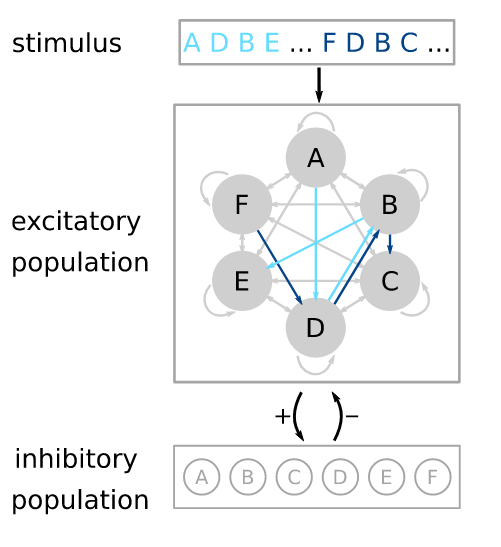
\includegraphics[width=0.6\textwidth]{model.png}

Younes Bouhadjar et al. | doi:10.1371/journal.pcbi.1010233
}
\column{0.5\textwidth}{
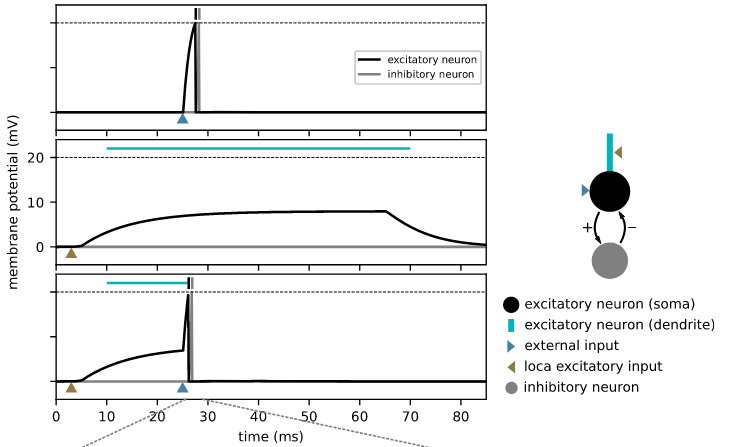
\includegraphics[width=0.9\textwidth]{excitatory_neuron_model.png}
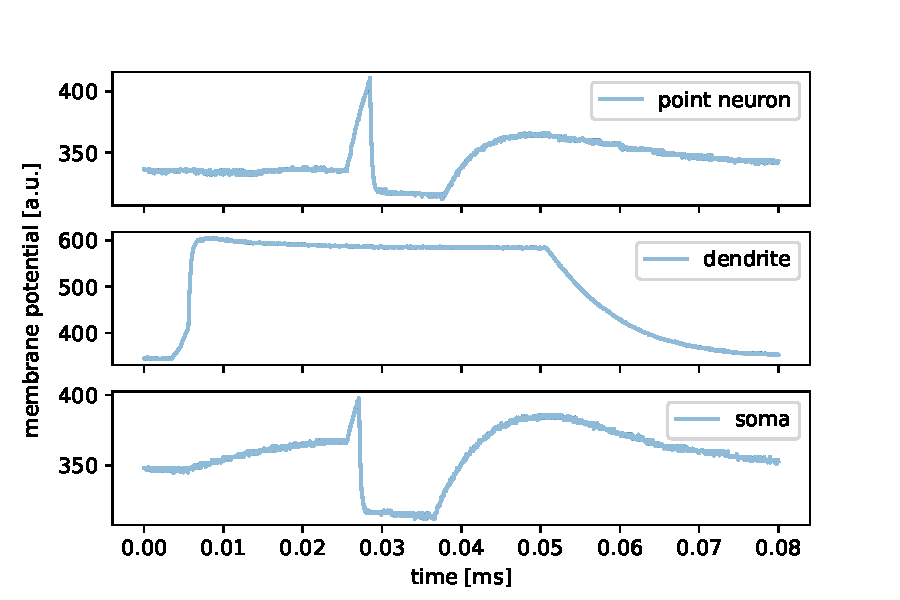
\includegraphics[width=0.65\textwidth]{../excitatory_neuron.pdf}
}
\end{columns}

\end{frame}

\begin{frame}{Towards HTM on BrainScaleS-2}

\begin{columns}
\column{0.5\textwidth}{
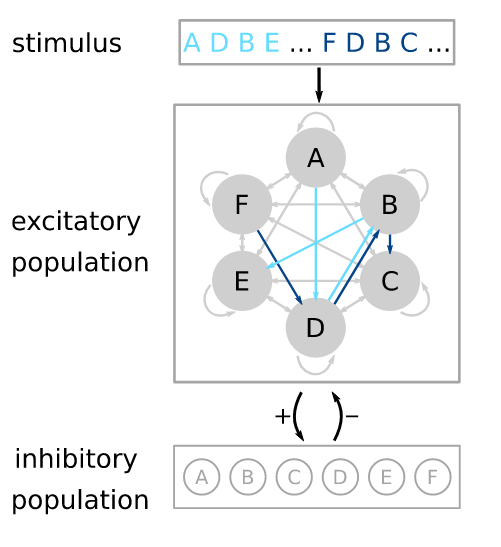
\includegraphics[width=0.6\textwidth]{model.png}

Younes Bouhadjar et al. | doi:10.1371/journal.pcbi.1010233
}
\column{0.5\textwidth}{
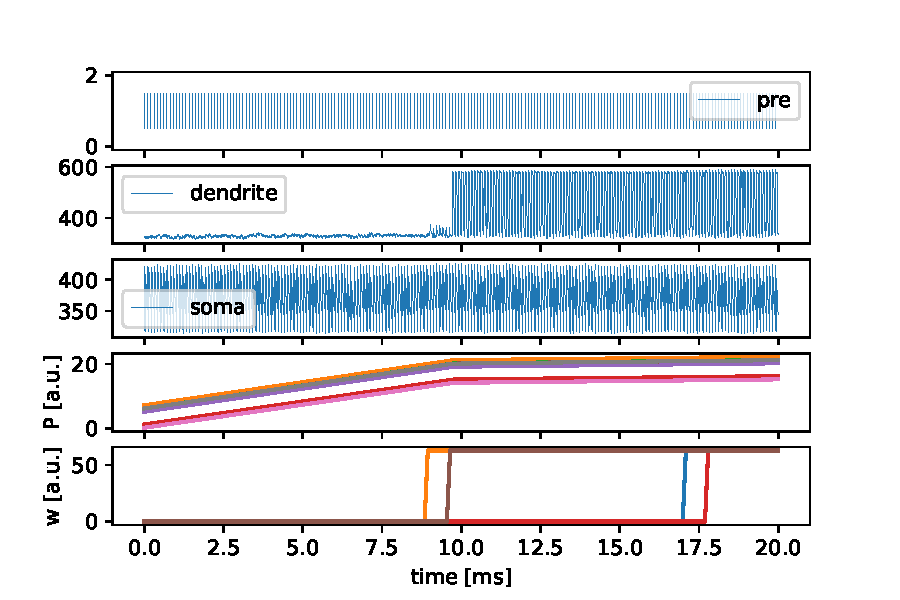
\includegraphics[width=\textwidth]{../plasticity.pdf}
\begin{itemize}
\item STDP \& homeostasis
\item binary weight state (mature or not)
\end{itemize}
}
\end{columns}

\end{frame}

\end{document}
